Eingereicht:

\begin{verbatim}[1, 3]\end{verbatim}

Gewählte Option 1 ist verfügbar?\begin{quote}Yes.\end{quote}Gewählte Option 3 ist verfügbar?\begin{quote}Yes.\end{quote}Anmerkungen zur eingereichten Lösung:

Alle angegebenen Klassendiagramme sind korrekt?

\begin{quote}\begin{verbatim}Nein.\end{verbatim}\end{quote}

Die korrekte Lösung ist:\begin{verbatim}[2,4]\end{verbatim}

Ihre Antwort zu Klassendiagramm 1 ist nicht richtig.

Klassendiagramm 1 ist ungültig.

Wenn es zum Beispiel die Vererbung, bei der E von B erbt, nicht gäbe, wäre es gültig.

Ihre Antwort zu Klassendiagramm 2 ist nicht richtig.

Klassendiagramm 2 ist gültig.

Die Beziehungen in dem Klassendiagramm könnten auf folgende Weise mit Namen versehen werden:



\begin{centering}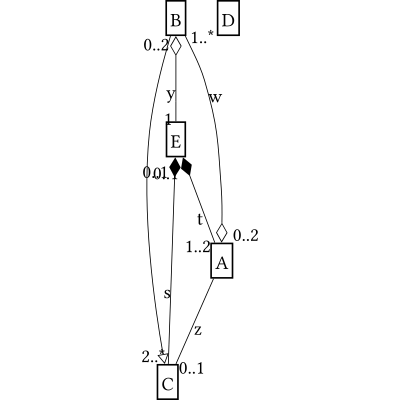
\includegraphics[min width=0.4\textwidth=0.6\textwidth,min height=0.4\textwidth=0.6\textwidth,keepaspectratio,max width=0.9\textwidth,max height=0.9\textwidth]{51/cd32786ed7955f75f2e4050d7464df637cf40075b2d129bb678089584e2eed975201af83b04c596701db35357ce8aed00a3a92e08161.pdf}\end{centering}



Betrachten Sie nun das folgende Objektdiagramm, welches eine Instanz dieses Klassendiagramms ist:



\begin{centering}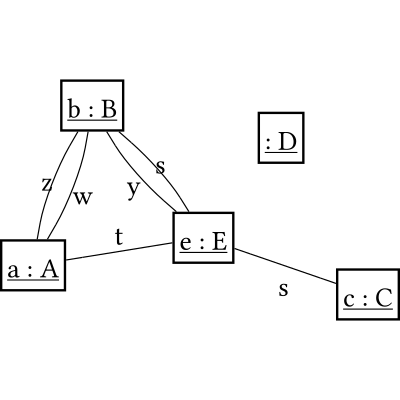
\includegraphics[min width=0.4\textwidth=0.6\textwidth,min height=0.4\textwidth=0.6\textwidth,keepaspectratio,max width=0.9\textwidth,max height=0.9\textwidth]{51/odcc69f5b1d023e969782ea5f974f3b12438efcf1e7d340bc3f501216ae3567bdf13.pdf}\end{centering}



Ihre Antwort zu Klassendiagramm 3 ist nicht richtig.

Klassendiagramm 3 ist ungültig.

Wenn es zum Beispiel die Vererbung, bei der E von B erbt, nicht gäbe, wäre es gültig.

Ihre Antwort zu Klassendiagramm 4 ist nicht richtig.

Klassendiagramm 4 ist gültig.

Die Beziehungen in dem Klassendiagramm könnten auf folgende Weise mit Namen versehen werden:



\begin{centering}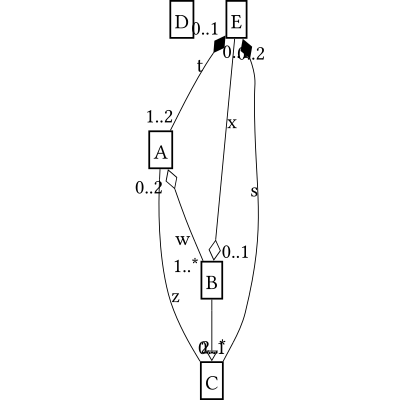
\includegraphics[min width=0.4\textwidth=0.6\textwidth,min height=0.4\textwidth=0.6\textwidth,keepaspectratio,max width=0.9\textwidth,max height=0.9\textwidth]{51/cd3faf14323c0cc9a0be4d24da2f2bee302bf2951cb8edca73b19f0e1599317b0301af83b04c596701db35357ce8aed00a3a92e08161.pdf}\end{centering}



Betrachten Sie nun das folgende Objektdiagramm, welches eine Instanz dieses Klassendiagramms ist:



\begin{centering}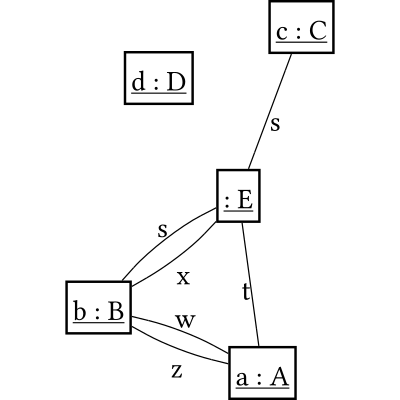
\includegraphics[min width=0.4\textwidth=0.6\textwidth,min height=0.4\textwidth=0.6\textwidth,keepaspectratio,max width=0.9\textwidth,max height=0.9\textwidth]{51/odbad91f15a5a868e5e1adda232caffabf7a2c51c009dd1f35b88c91083fb9330013.pdf}\end{centering}



